\chapter{Rasprava i budući rad}
\label{ch:discussion_future_work}

\selectlanguage{croatian}

Rezultati evaluacije i praktična iskustva s implementiranim sustavom otvaraju prostor za dublju analizu postignutih rezultata, identificiranih ograničenja te smjernica za buduća istraživanja. Ovo poglavlje kritički analizira trenutno stanje sustava i predlaže konkretne pravce daljnjeg razvoja.

\section{Ograničenja}

Unatoč postignućima u omogućavanju pristupa otvorenim podacima kroz prirodni jezik, sustav se suočava s nekoliko ključnih ograničenja koja utječu na njegovu primjenjivost u produkcijskom okruženju.

\subsection{Ovisnost o komercijalnim LLM API-jima}

Trenutna implementacija oslanja se na OpenAI GPT-4 model za generiranje SPARQL upita, što uvodi nekoliko izazova:

\subsubsection{Latencija i performanse}

Pozivi prema OpenAI API-ju čine 38.6\% ukupnog vremena odziva sustava. Ova latencija uključuje:

\begin{itemize}
    \item \textbf{Mrežnu latenciju}: 500-800ms ovisno o geografskoj lokaciji
    \item \textbf{Vrijeme obrade na serveru}: 2-3s za složenije \textit{prompt}-ove
    \item \textbf{Queue vrijeme}: Dodatnih 0-2s tijekom vršnih opterećenja
\end{itemize}

Latencija je posebno problematična za:
\begin{itemize}
    \item Interaktivne aplikacije koje zahtijevaju brz odziv
    \item Scenarije s velikim brojem istovremenih korisnika
    \item Korisnike s sporijim internetskim vezama
    \item Aplikacije koje zahtijevaju predvidljivo vrijeme odziva
\end{itemize}

\subsubsection{Troškovi skaliranja}

Ekonomski aspekt korištenja komercijalnih API-ja postaje značajan pri većem broju korisnika:

\begin{table}[htbp]
\centering
\caption{Projekcija troškova za različite razine korištenja}
\label{tab:cost_projection}
\begin{tabular}{|l|c|c|c|}
\hline
\textbf{Razina korištenja} & \textbf{Upita/mjesec} & \textbf{Trošak/upit} & \textbf{Mjesečni trošak} \\
\hline
Pilot projekt & 1,000 & \$0.08 & \$80 \\
Mala organizacija & 10,000 & \$0.08 & \$800 \\
Srednja organizacija & 50,000 & \$0.08 & \$4,000 \\
Nacionalni portal & 200,000 & \$0.08 & \$16,000 \\
EU razina & 1,000,000 & \$0.08 & \$80,000 \\
\hline
\end{tabular}
\end{table}

Troškovi mogu biti prohibitivni za:
\begin{itemize}
    \item Javne institucije s ograničenim budžetima
    \item Neprofitne organizacije
    \item Obrazovne ustanove
    \item Projekte otvorenog koda
\end{itemize}

\subsubsection{Sigurnosni i privatnosti aspekti}

Slanje korisničkih upita vanjskim API-jima uvodi zabrinutosti vezane uz:

\begin{itemize}
    \item \textbf{Privatnost podataka}: Upiti se obrađuju kod treće strane
    \item \textbf{Usklađenost s GDPR}: Pitanja vezana uz obradu osobnih podataka
    \item \textbf{Korporativna sigurnost}: Potencijalno curenje osjetljivih informacija
    \item \textbf{Geopolitička ograničenja}: Neki regioni mogu imati restrikcije
\end{itemize}

\subsection{Jezična podrška}

Trenutna implementacija pokazuje najbolje rezultate za upite na engleskom jeziku, što predstavlja barijeru za širu primjenu u europskom kontekstu.

\subsubsection{Izazovi s hrvatskim jezikom}

Testiranje s upitima na hrvatskom jeziku pokazuje:

\begin{itemize}
    \item \textbf{Smanjena točnost}: 73\% uspjeha nasuprot 92\% za engleski
    \item \textbf{Problemi s dijakritičkim znakovima}: č, ć, ž, š, đ često uzrokuju greške
    \item \textbf{Gramatička složenost}: Padeži i glagolski oblici zbunjuju model
    \item \textbf{Nedostatak primjera}: Manje kvalitetnih primjera za trening
\end{itemize}

\subsubsection{Višejezični kontekst EU}

EU Portal podataka sadrži metapodatke na 24 službena jezika, što zahtijeva:

\begin{itemize}
    \item Podršku za \textit{cross-lingual} pretraživanje
    \item Razumijevanje kulturoloških razlika u terminologiji
    \item Rukovanje miješanim jezičnim upitima
    \item Održavanje konzistentnosti kroz jezike
\end{itemize}

\subsection{Skalabilnost sustava}

Evaluacija pokazuje degradaciju performansi pri više od 10 istovremenih korisnika, što ograničava primjenjivost za veće organizacije.

\subsubsection{Identificirana uska grla}

\begin{enumerate}
    \item \textbf{CPU intenzivnost generiranja \textit{embeddings}-a}:
    \begin{itemize}
        \item Jedan CPU \textit{thread} po upitu
        \item 200-300ms po \textit{embedding}-u
        \item Linearno skaliranje s brojem upita
    \end{itemize}
    
    \item \textbf{Memorijski zahtjevi ChromaDB}:
    \begin{itemize}
        \item 2GB bazna potrošnja
        \item +500MB po 10,000 vektora
        \item Eksponencijalni rast za velike kolekcije
    \end{itemize}
    
    \item \textbf{API rate limiti}:
    \begin{itemize}
        \item OpenAI: 10,000 tokena/min
        \item SPARQL endpoint: 10 upita/s
        \item CKAN API: 100 zahtjeva/min
    \end{itemize}
\end{enumerate}

\subsubsection{Arhitekturalna ograničenja}

Trenutna monolitna arhitektura otežava:

\begin{itemize}
    \item Horizontalno skaliranje komponenti
    \item Load balancing između instanci
    \item Geografsku distribuciju
    \item Fault tolerance i high availability
\end{itemize}

\subsection{Domensko usmjeravanje}

Sustav je optimiziran specifično za EU Portal otvorenih podataka i DCAT standard, što ograničava njegovu primjenjivost na druge domene.

\subsubsection{Vezanost uz DCAT}

Trenutna implementacija pretpostavlja:

\begin{itemize}
    \item DCAT-AP 2.0.1 strukturu metapodataka
    \item Specifične SPARQL \textit{endpoint} karakteristike
    \item EU tematske taksonomije
    \item Standardizirane kontrolirane vokabulare
\end{itemize}

Prilagodba drugim standardima (npr. Schema.org, VOID) zahtijeva:
\begin{itemize}
    \item Ponovno treniranje modela
    \item Prilagodbu ekstrakcije sheme
    \item Nove primjere upita
    \item Modificirane validacijske logike
\end{itemize}

\subsubsection{Nedostatak domenskog znanja}

Za specijalizirane domene (medicina, pravo, financije) sustav pokazuje:

\begin{itemize}
    \item Nerazumijevanje stručne terminologije
    \item Generiranje semantički neispravnih upita
    \item Propuštanje važnih domenskih ograničenja
    \item Nemogućnost inferiranja implicitnih veza
\end{itemize}

\section{Smjernice za buduća istraživanja}

Na temelju identificiranih ograničenja i praktičnih iskustava, predlažemo nekoliko konkretnih pravaca za daljnji razvoj sustava.

\subsection{Implementacija lokalnih LLM-ova}

Prelazak na lokalno pokretane jezične modele predstavlja ključnu strategiju za rješavanje problema latencije, troškova i privatnosti.

\subsubsection{Kandidati za lokalne modele}

Nekoliko \textit{open source} modela pokazuje obećavajuće rezultate:

\begin{table}[htbp]
\centering
\caption{Usporedba lokalnih LLM kandidata}
\label{tab:local_llm_comparison}
\begin{tabular}{|l|c|c|c|c|}
\hline
\textbf{Model} & \textbf{Parametri} & \textbf{VRAM} & \textbf{Točnost} & \textbf{Brzina} \\
\hline
Llama 3 70B & 70B & 140GB & 85\% & Spora \\
Llama 3 8B & 8B & 16GB & 76\% & Brza \\
Mixtral 8x7B & 47B & 94GB & 82\% & Srednja \\
CodeLlama 34B & 34B & 68GB & 88\% & Srednja \\
Mistral 7B & 7B & 14GB & 74\% & Vrlo brza \\
\hline
\end{tabular}
\end{table}

\subsubsection{Strategija implementacije}

Predloženi pristup za implementaciju:

\begin{enumerate}
    \item \textbf{Hibridni model}:
    \begin{itemize}
        \item Lokalni model za jednostavne upite (70\% slučajeva)
        \item GPT-4 fallback za kompleksne upite
        \item Dinamičko usmjeravanje na temelju složenosti
    \end{itemize}
    
    \item \textbf{Fine-tuning strategija}:
    \begin{itemize}
        \item Prikupiti 10,000+ uspješnih SPARQL generiranja
        \item Fine-tune CodeLlama modela specifično za SPARQL
        \item Kontinuirano učenje iz produkcijskih podataka
    \end{itemize}
    
    \item \textbf{Optimizacija inferiranja}:
    \begin{itemize}
        \item Kvantizacija modela (8-bit, 4-bit)
        \item Model sharding kroz više GPU-a
        \item Batch inferiranje za bolju iskoristivost
        \item TensorRT ili ONNX optimizacije
    \end{itemize}
\end{enumerate}

\subsubsection{Očekivane prednosti}

Implementacija lokalnih modela omogućila bi:

\begin{itemize}
    \item \textbf{Smanjenje latencije}: <1s za generiranje upita
    \item \textbf{Eliminacija troškova}: Nakon početne investicije
    \item \textbf{Potpuna kontrola}: Nad podacima i procesom
    \item \textbf{Prilagodljivost}: Specifična optimizacija za domenu
\end{itemize}

\subsection{Unapređenje baze primjera}

Kontinuirano proširivanje i poboljšanje vektorske baze primjera ključno je za održavanje i poboljšanje točnosti sustava.

\subsubsection{Strategija aktivnog učenja}

Implementacija \textit{active learning} pristupa:

\begin{enumerate}
    \item \textbf{Automatsko prikupljanje}:
    \begin{itemize}
        \item Svaki uspješan upit dodaje se u bazu
        \item Automatska evaluacija kvalitete rezultata
        \item A/B testiranje različitih formulacija
    \end{itemize}
    
    \item \textbf{Kuriranje primjera}:
    \begin{itemize}
        \item Stručna validacija kompleksnih upita
        \item Uklanjanje redundantnih primjera
        \item Balansiranje po domenama i složenosti
    \end{itemize}
    
    \item \textbf{Sintetičko generiranje}:
    \begin{itemize}
        \item LLM generira varijacije postojećih upita
        \item Automatska validacija kroz izvršavanje
        \item Augmentacija rijetkih tipova upita
    \end{itemize}
\end{enumerate}

\subsubsection{Optimizacija vektorskog prostora}

Poboljšanja u organizaciji vektorske baze:

\begin{itemize}
    \item \textbf{Hijerarhijsko klasteriranje}: Grupiranje sličnih upita
    \item \textbf{Dinamički k-NN}: Prilagođavanje broja susjeda složenosti
    \item \textbf{Temporal weighting}: Noviji primjeri imaju veću težinu
    \item \textbf{Domain-specific embeddings}: Specijalizirani modeli po domenama
\end{itemize}

\subsection{Bolje strategije sinteze}

Trenutna sinteza rezultata može se unaprijediti kroz sofisticiranije tehnike.

\subsubsection{Algoritmi rangiranja}

Implementacija algoritama rangiranja:

\begin{enumerate}
    \item \textbf{Learning to Rank}:
    \begin{itemize}
        \item Treniranje modela na sistemskim interakcijama
        \item Adaptivno rangiranje rezultata
        \item Kontekstualni faktori (vrijeme, lokacija)
    \end{itemize}
    
    \item \textbf{Multi-criteria optimization}:
    \begin{itemize}
        \item Relevantnost + aktualnost + kvaliteta
        \item Pareto-optimalno rangiranje
        \item Eksplicitne sistemske preferencije
    \end{itemize}
    
    \item \textbf{Eksplanatorno rangiranje}:
    \begin{itemize}
        \item Objašnjenje zašto je rezultat visoko rangiran
        \item Vizualizacija faktora rangiranja
        \item Interaktivno prilagođavanje težina
    \end{itemize}
\end{enumerate}

\subsubsection{Kombiniranje rezultata}

Tehnike za kombiniranje rezultata:

\begin{itemize}
    \item \textbf{Entity resolution}: Prepoznavanje istih entiteta
    \item \textbf{Relationship extraction}: Otkrivanje veza između skupova
    \item \textbf{Temporal alignment}: Usklađivanje vremenskih serija
    \item \textbf{Conflict resolution}: Rukovanje kontradiktornim podacima
\end{itemize}

\subsection{Višejezična podrška}

Razvoj potpune višejezične podrške ključan je za europski kontekst.

\subsubsection{Arhitektura za višejezičnost}

Predložena arhitektura uključuje:

\begin{enumerate}
    \item \textbf{Multilingual embeddings}:
    \begin{itemize}
        \item Modeli trenirani na 100+ jezika
        \item Zajednički vektorski prostor
        \item Cross-lingual similarity
    \end{itemize}
    
    \item \textbf{Language-agnostic SPARQL}:
    \begin{itemize}
        \item Generiranje neovisno o jeziku upita
        \item Automatska translacija labela
        \item Podrška za višejezične rezultate
    \end{itemize}
    
    \item \textbf{Lokalizacija sučelja}:
    \begin{itemize}
        \item Prijevodi svih UI elemenata
        \item Kulturološki prilagođeni primjeri
        \item Lokalne konvencije za datume/brojeve
    \end{itemize}
\end{enumerate}

\subsubsection{Hrvatski jezik specifično}

Za potpunu podršku hrvatskog jezika potrebno je:

\begin{itemize}
    \item Fine-tuning modela na hrvatskim tekstovima
    \item Građenje korpusa hrvatskih SPARQL primjera
    \item Integracija s hrvatskim jezičnim resursima
    \item Podrška za dijalekte i regionalizme
\end{itemize}

\subsection{Prelazak na distribuiranu arhitekturu}

Prelazak na mikroservisnu arhitekturu omogućio bi bolje skaliranje.

\subsubsection{Predložena mikroservisna arhitektura}

\begin{figure}[htbp]
    \centering
    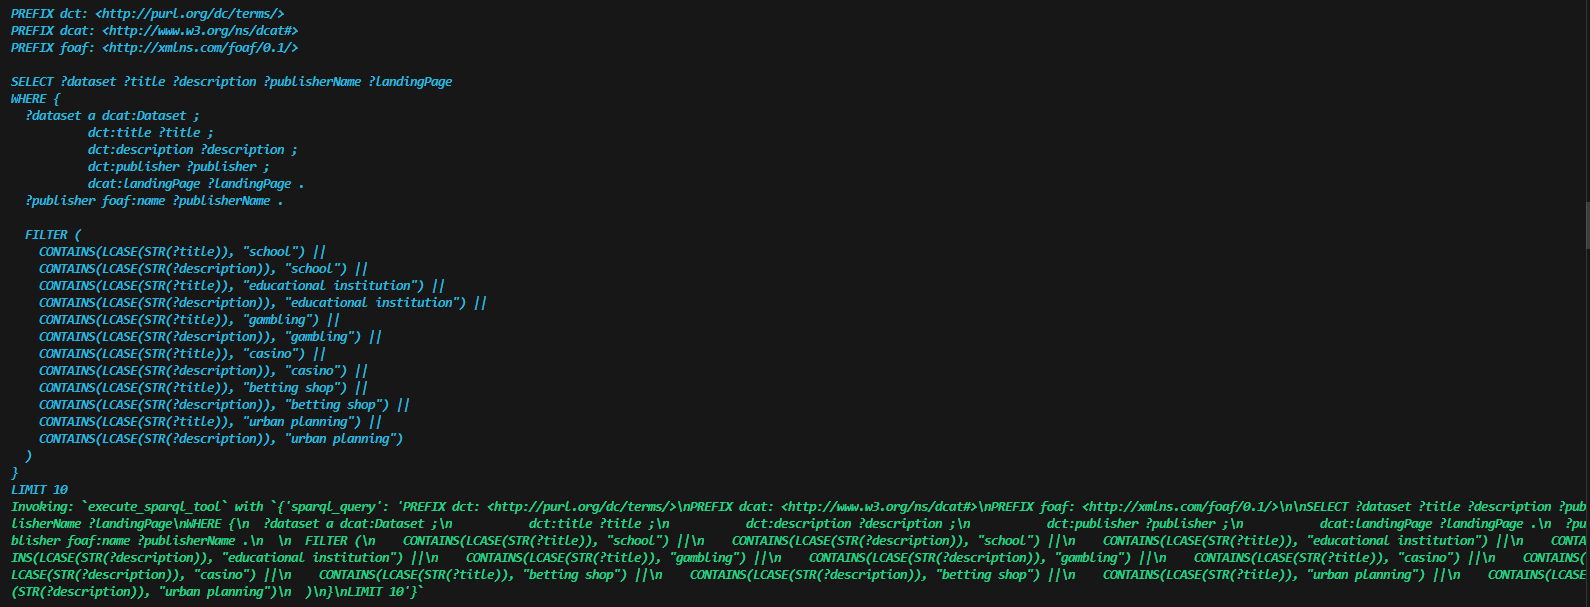
\includegraphics[width=1\textwidth]{figures/izvjestaj_image_82.png}
    \caption{Predložena mikroservisna arhitektura za skalabilnost}
    \label{fig:microservices_architecture}
\end{figure}

Ključne komponente:

\begin{enumerate}
    \item \textbf{API Gateway}: Load balancing i routing
    \item \textbf{Query Service}: Upravljanje korisničkim upitima
    \item \textbf{Embedding Service}: Generiranje vektorskih reprezentacija
    \item \textbf{Vector DB Cluster}: Distribuirana vektorska baza
    \item \textbf{SPARQL Generator}: Pool LLM instanci
    \item \textbf{Result Aggregator}: Kombiniranje rezultata
    \item \textbf{Cache Layer}: Distribuirani Redis cache
\end{enumerate}

\subsubsection{Prednosti distribuirane arhitekture}

\begin{itemize}
    \item \textbf{Horizontalno skaliranje}: Svaki servis nezavisno
    \item \textbf{Fault tolerance}: Redundancija kritičnih komponenti
    \item \textbf{Geografska distribucija}: Servisi bliže korisnicima
    \item \textbf{Resource optimization}: Različiti resursi po servisu
    \item \textbf{Independent deployment}: Ažuriranja bez prekida
\end{itemize}

\subsection{Dodatne značajke korisničkog sučelja}

Sučelje sustava može se proširiti kroz dodatne značajke.

\subsubsection{Vizualizacija podataka}

Automatsko generiranje vizualizacija:

\begin{itemize}
    \item \textbf{Grafovi}: Za vremenske serije i trendove
    \item \textbf{Geografske karte}: Za prostorne podatke
    \item \textbf{Mreže}: Za prikaz relacija
    \item \textbf{Dashboardi}: Za kompleksne analize
\end{itemize}

\subsubsection{Interaktivno istraživanje}

Omogućavanje iterativnog pristupa:

\begin{itemize}
    \item \textbf{Query refinement}: Postupno usavršavanje upita
    \item \textbf{Faceted search}: Filtriranje rezultata
    \item \textbf{Related queries}: Sugestije sličnih upita
    \item \textbf{Query history}: Praćenje aktivnih sesija
\end{itemize}

\subsubsection{Kolaborativne značajke}

Podrška za timski rad:

\begin{itemize}
    \item \textbf{Dijeljenje upita}: URL za reprodukciju
    \item \textbf{Anotacije}: Komentari na rezultate
    \item \textbf{Workspaces}: Organizacija projekata
    \item \textbf{Version control}: Praćenje promjena upita
\end{itemize}

\section{Dugoročna vizija}

Dugoročno, sustav ima potencijal evoluirati u sveobuhvatnu platformu za demokratizaciju pristupa podacima.

\subsection{Integracija s AI ekosistemom}

Povezivanje s drugim AI alatima:

\begin{itemize}
    \item \textbf{AutoML}: Automatska analiza podataka
    \item \textbf{NLP pipeline}: Ekstrakcija znanja iz dokumenata
    \item \textbf{Computer vision}: Analiza vizualnih podataka
    \item \textbf{Predictive analytics}: Prognoziranje trendova
\end{itemize}

\subsection{Standardizacija pristupa}

Razvoj standarda za:

\begin{itemize}
    \item Natural language to SPARQL mapping
    \item Cross-portal query federation
    \item Semantic search APIs
    \item Quality metrics za otvorene podatke
\end{itemize}

\subsection{Edukacijska komponenta}

Integracija edukacijskih elemenata:

\begin{itemize}
    \item Interaktivni SPARQL tutoriali
    \item Objašnjenja generiranih upita
    \item Best practices za podatke
    \item Certificiranje data literacy
\end{itemize}

Ova dugoročna vizija pozicionira sustav ne samo kao alat za pristup podacima, već kao platformu za podizanje razine podatkovne pismenosti i omogućavanje inovacija temeljenih na otvorenim podacima. 